\section{Actividad No 01 – Sistema Control de Versiones} 

\begin{itemize} % CREA GUIONES
\item \textbf{¿Que es un Sistema Control de Versiones?}\\

Un sistema de control de versiones (SCV) es una herramienta que nos permite el registro de todos los cambios hechos en uno o más proyectos, guardando así todas las versiones del producto en todas sus fases de desarrollo.
	
En un sistema control de versiones,las versiones son como fotografías que registran su estado actual en ese momento del tiempo y se van guardando a medida que se hacen modificaciones al código fuente.
	
Otros autores lo definen como un software que controla y organiza las
distintas revisiones que se realizen sobre uno o varios documentos,como los cambios realizados sobre un documento,
por ejemplo añadir un parrafo, borrar un fragmento o algo similar.\\

EJEMPLO:\\

En un principio se carga el siguiente codigo:\\

\begin{center}
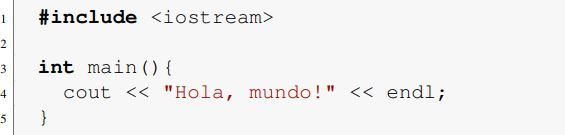
\includegraphics[width=12cm]{./Imagenes/actividad0101} 
\end{center}
	
Donde el SCV lo almacena como la version 1 del proyecto, de manera que si realizamos cambios se quedara almacenado por versiones.\\
	
Si quisieramos modificar el codigo por algún error que haya surgido,lo modificariamos de la siguiente manera:\\

\begin{center}
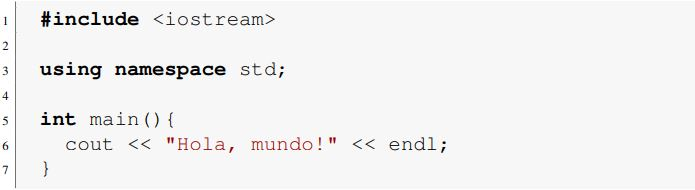
\includegraphics[width=13cm]{./Imagenes/actividad0102} 
\end{center}
	
Añadiendolo al SCV,este lo almacenara como la version 2 del proyecto,de manera que podamos tener todas las versiones de los cambios que se hayan hecho en el proyecto durante su tiempo de desarrollo.\\
\end{itemize} 


\begin{itemize}
\item \textbf{Caracteristicas de un Sistema Control de Versiones:} \\

Un sistema de control de versiones debe proporcionar:\\

\begin{enumerate}[1.] % CREA ENUMERACION
\item Mecanismo de almacenamiento de los elementos que deba gestionar.
\item Posibilidad de realizar cambios sobre los elementos almacenados.
\item Registro histórico de las acciones realizadas con cada elemento o conjunto de elementos.\\
\end{enumerate}
\end{itemize} 


\begin{itemize}
\item \textbf{Clasificacion de un Sistema Control de Versiones:} \\

Los sistemas de control de versiones se pueden clasifica en 2 grandes grupos:\\

\begin{enumerate}[1.] % CREA ENUMERACION
\item Centralizados\\

En un sistema de control de versiones centralizado todos nuestros fuentes y sus versiones están almacenados en un único directorio de un ordenador. Todos los desarrolladores que quieran trabajar con esos fuentes, deben pedirle al sistema de control de versiones una copia local para trabajar. En ella realizan todos sus cambios y cuando están listos y funcionando, le dicen al sistema de control de versiones que guarde los fuentes modificados como una nueva versión.\\

\item Distribuidos\\

En un sistema de control de versiones distribuido no hay un repositorio central. Todos los desarrolladores tienen su propia copia del repositorio, con todas las versiones y toda la historia. Según van desarrollando y haciendo cambios, sus fuentes y versiones van siendo distintas unas de otras.\\
\end{enumerate}
\end{itemize} 


\begin{itemize}
\item \textbf{Funcionamiento de un Sistema Control de Versiones:} \\

Todos los sistemas de control de versiones se basan en disponer de un repositorio, que es el conjunto de información gestionada por el sistema. Este repositorio contiene el historial de versiones de todos los elementos gestionados.

Cada uno de los usuarios puede crearse una copia local duplicando el contenido del repositorio para permitir su uso. Para modificar la copia local existen dos semánticas básicas:\\

\begin{enumerate}[1.] % CREA ENUMERACION
\item Exclusivos

Para poder realizar un cambio es necesario marcar en el repositorio el elemento que se desea modificar y el sistema se encargará de impedir que otro usuario pueda modificar dicho elemento.\\

\item Colaborativos

En el que cada usuario se descarga la copia, la modifica, y el sistema automáticamente combina las diversas modificaciones. Puede estar sujeto a la aparición de conflictos que deben ser solucionados manualmente.\\
\end{enumerate}
\end{itemize} 

